%%%%%%%%%%%%%%%%%%%%%%%%%%%%%%%%%%%%%%%%%%%%%%%%%%%%%%%%%%%%%%%%%%%%%%%%%%%%%%%%

\section{Popis problému}
\label{sec_problem_description}

V~současné době je již většina internetového provozu šifrována~\cite{bib_matousek}. Jakkoliv šifrování zvyšuje bezpečnost a soukromí uživatelů, znesnadňuje na druhou stranu monitorovací a analytickou činnost. Tento projekt se zaměřuje na jednu z~možných technik rozpoznávání aplikací v~šifrovaném TLS (\textit{Transport Layer Security}) provozu. Jsme omezeni výhradně na komunikaci mobilních platforem.

TLS je protokol, který pracuje nad TCP, kde zajišťuje soukromí a integritu dat pro komunikaci aplikací. Navázání TLS spojení probíhá pomocí tzv. TLS \textit{handshake}. V~této fázi komunikace jsou mezi klientem a serverem vyjednány informace o~způsobu šifrování~--~metody pro výměnu klíčů, šifrovací algoritmy, verze, výměna šifrovacích klíčů, autentizace, apod~\cite{bib_matousek}. Tato fáze komunikace probíhá pochopitelně nešifrovaně, veškerý další provoz již šifrovaný je.

\begin{figure}[H]
    \centering
    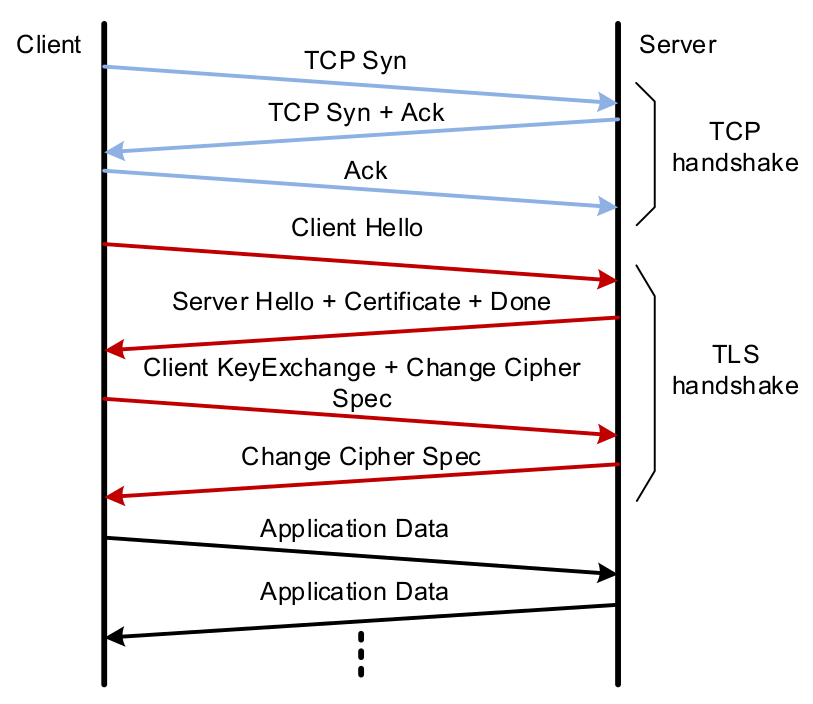
\includegraphics[width=0.8\linewidth]{tls.png}
    \caption{Ustanovení TLS spojení. Obrázek je převzatý~\cite{bib_matousek}.}
    \label{fig_tls}
\end{figure}

%%%%%%%%%%%%%%%%%%%%%%%%%%%%%%%%%%%%%%%%%%%%%%%%%%%%%%%%%%%%%%%%%%%%%%%%%%%%%%%%
